\documentclass[main.tex]{subfiles}

\begin{document}
\section{Данни и резултати}

Наличните бази данни за ЕЕГ са много по-малко от тези за реч. Това вероятно се дължи на факта, че съставянето им е доста по-трудно. Освен че изискват специална апаратура (тоест електроенцефалограф), изискванията към постановката са много по-строги. Тъй като се цели при записа да има възможно най-малко дразнители, освен представения от експеримента, трябва да се подсигури, че субектът е седнал удобно, на определено разстояние от монитора, не е болен, не му е студено или топло, не мига (или е със затворени очи), не говори и като цяло се движи възможно най-малко. Ако нещо в постановката се наруши, например човекът е мигнал, се трие целият запис. Често се подсигурява да не е бил консумиран кофеин (поне от страна на субекта, но вероятно е препоръчително и от страна на учения) в последните 24 часа и човекът да е имал нормален цикъл на съня. Допълнителна информация от типа дали субектът пуши, дали е левичар или десничар и какъв е по професия, се съобщава, тъй като не се знае дали не влияе на експеримента по някакъв начин. 

Целта на тази дипломна работа обаче е да се изследва комбинирането на сигнал от реч и ЕЕГ сигнал. Това изисква да имаме такава постановка, при която човекът говори, докато е свързан към електроенцефалограф, за да имаме данни от двата сигнали в един същи момент от време. Ако мигането е забранено, то комплексна дейност като говоренето е направо еретична за наличните бази данни. Поради тази причина, и поради липсата\footnote{до колкото ми е известно} на подходяща база, такава трябваше да бъде създадена за конкретните цели.

Идеята е да се съчетаят най-често използваните похвати за създаване на емоционална речева база от една страна и емоциална ЕЕГ база от друга.

За реч най-често се използва една от следните две постановки: субектите (най-често актьори) четат предварително избрани емоционални изречения; субектите разказват емоционална случка по свой избор, например нещо преживяно или прочетено.

За ЕЕГ най-често се използва един от следните стимули: гледане на специално подбрани емоционални картинки\footnote{Например \url{https://web.archive.org/save/https://csea.phhp.ufl.edu/media/iapsmessage.html}}; слушане на специално подбрана емоционална музика; гледане на специално избрани емоционалени клипчета.

Първият опит за емоционална база данни целеше резултатът да е възможно най-близък до съществуващите вече бази и се състои от две части.
В първата част се гледат 15 специално избрани картинки (5 положителни, 5 отрицателни, 5 неутрални), като между картинките има пауза с черен ектран. След това започва втората фаза, като на екрана се показва обяснение за протичането ѝ. Показва се произволно емоционално клипче (със средна дължина от една минута), субектът описва какво е видял на клипчето в продължение на десет секунди и след това чете показан на екрана текст.
Клипчетата са 3 за щастие, 3 за тъга и 3 за гняв, а текстовете са подбрани от прогнозата за времето. Счита се, че четенето на прогнозата за времето ще произведе неутрални данни.
Субектът предварително знае постановката на опита.

\begin{figure}[ht]%
    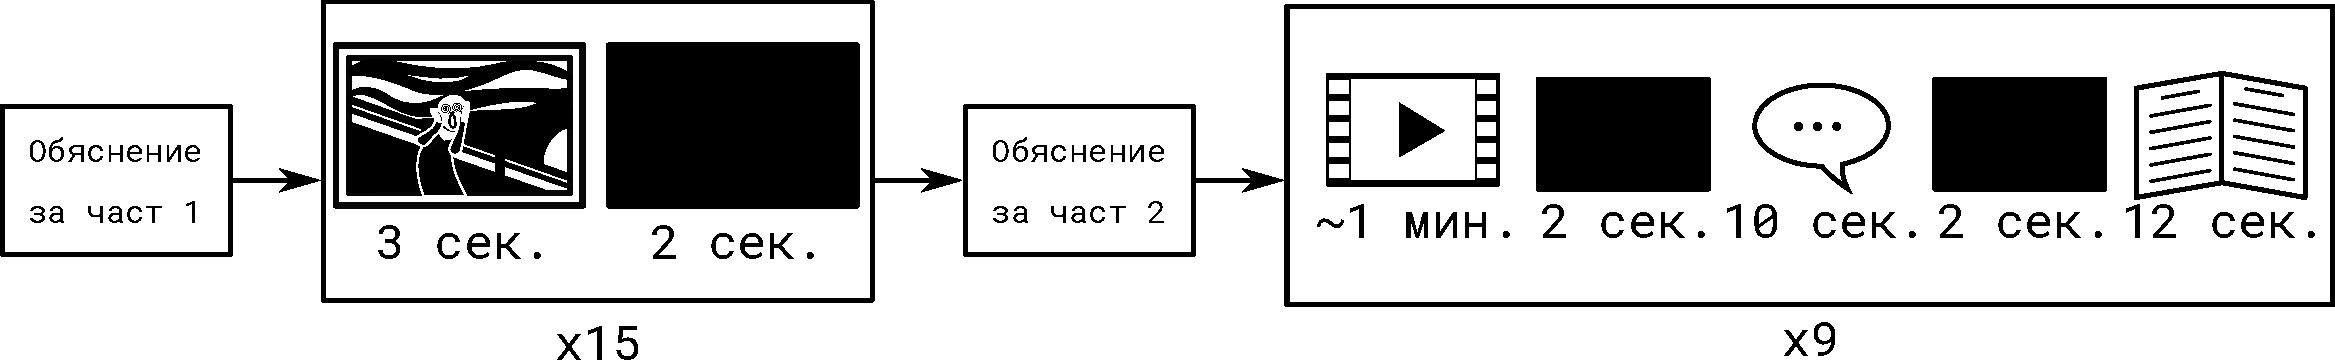
\includegraphics[width=\textwidth]{first_db}%
    \label{fig:brain_res:1}
\end{figure}

След експеримента първият и единствен субект сподели, че видеата не са успели да предизвикат искрена емоция. Оказва се, че периодът от 1-2 минути, през който се гледа видео, е твърде кратък, за да може да се събуди непринудена емоционална реакция, ако видеата не са специално избрани с предварително знание за конкретния субект. Вероятно може да се постигне желания ефект, ако гледаните видеа са достатъчно дълги, за да може субектът да развие емоционална привързаност, например с дължината на филм. За съжаление обаче, използването на мокри електроди позволява максимална продължителност на целия експеримент около 10-15 минути, след което време соления разтвор по електродите изсъхва и съпротивлението им става твърде голямо, за да може да ги отчете уредът. 

Всъщност най-големият проблем е, че емоциите имат твърде различен характер и заради това се предизвикват и изразяват по различен начин. Щастието се предизвиква по-лесно от гнева чрез визуални стимули. Гневът обикновено изисква субектът да има лично отношение към темата, която му се представя. Щастието има много по-момента изява от тъгата, която се развива продължително. Като цяло емоциите с ниска енергия се изразяват много по-трудно вербално от тези с висока. 
Мисля, че генерално не знам какво искам да кажа.

Започнах да си мисля, че вместо да се опитвам да намеря универсални за всички хора клипчета, мога намеря разбиване на типовече хора, спрямо начинът, по който може да се предизвика емоция у тях. Например ако вземем класификацията на Юнг, в която всеки човек попада в една от 16 категории в зависимост къде стои по четирите оси: интровертен-екстровертен, наблюдаващ-интуитивен,  чувстващ-мислещ, съдещ-приемащ (в зависимост от какво прави с наличната си информация). Дали ако двама човека попадат в една и съща категория, ще може емоцията да се предизвика (и евентуално изрази) по сходен начин. Съставих анкета, която цели да провери какъв тип стимул а нужен за предизвикването на всяка една от емоциите и какви клипчета предизвикват емоционална реакция у участниците. Първо, за всяка една от изследваните емоции се се търси най-подхдяшия начин за предизвикването ѝ, като възможностите са:
\begin{enumerate}
    \item Текст
    \item Видео
    \item Разговор
    \item Картинка
    \item Медията няма значение, само контекстът
\end{enumerate}
Участниците имат право да избират повече от един отговор.

Отговорите показват, че докато тъгата може да бъде предизвикана чрез пасивни методи - най-честият отговор е текст - щастието и тъгата се предизвикват по-лесно в социална обстановка (чрез разговор). Също така в малката извадка от пет участника, категориите на Юнг не носят информация за емоциалното възприемане на стимулите.

Във втората част на анкетата резултатите стават още по-объркани. Там участниците са помолени да изберат видео, картинка, текст или да опишат нещо, което ги предразполага емоционално. Оказва се, че предизвикването на емоция е твърде лично и няма засичащи се теми измежду всички отговори.

Последната част на анкетата не донесе допълнителен успех. В нея на участниците са представени стимули (видеа и картинки), в които трябва да бъде определен сантимента измежду неутрално, щастие, тъга, гняв. Отново, отговорите не съвпадат върху нито един стимул.

Заключението е, че нещата, които предизвикват емоция, са твърде индивидуални. Всъщност според някои психолози (\cite{stupid-book}), емоциите изобщо не са универсални, а напротив - те са изцяло социална констуркция. Това означава, че ако участниците са от различен социален кръг (различна възраст, условия на живот, интереси), има малък шанс да имат сходен начин за изразяването на емоциите им. Дори да се доверим на класическата теория, че шаблон на емоциите съществува, все още не знам как избера видеа, които биха предизвикали емоция у повече от един участник.

Този негативен опит вдъхнови втория опит. При него емоцията се предизвиква от лични преживявания. Първоначалното нежелание да използва този метод, е свързан с липсата на равни условия между участниците, тъй като избраният стимул зависи от самия участник. Тъй като различните хора са различно емпатични към предварително избраните стимули обаче (ако са изобщо), то тази постановка може да се доближава повече до генерирането на искрено емоционални данни.

Вторият опит се отдалечава повече от стандартните постановки, тъй като използва множество различни дразнители, тъй като цели да предразположи максимално субекта, според неговите нужди. Дава му се възможност да избере видеа, които му действат емоционално. Дава се възможност за слушане на аудио запис през времето на експеримента. Останалата част протича просто: субектът си избира емоцията и по негово желание може да включва стимули. При натискане на бутон ``Enter'' се пуска видео от предварително избраните, натискане на бутон ``Space'' означава съответно начало и край на аудио запис, през който субектът е свободен да говори каквото си избере. В експеримента няма времеви ограничения или минимален брой записи, които субектът трябва да направи, нито определена тема. След първите петнайсет минути, експериментът се прекъсва (ако е продължил толкова дълго), тъй като електродите изсъхват. В експериментът е намесено много движение от страна на субекта, тъй като се изисква да натиска бутони.

\begin{table}[h]
    \begin{center}
    \begin{tabular}{|l|r|r|} 
        \hline
        Емоция & Брой файлове & Обща дължина\\ 
        \hline
        Гняв & 3 & 0 мин. 30 сек.\\ 
        Щастие & 3 & 0 мин. 30 сек.\\ 
        Неутрално състояние & 10 & 2 мин. 00 сек. \\ 
        Тъга & 4 & 0 мин. 40 сек. \\ 
        \hline
    \end{tabular}
    \caption{Дължина и брой файлове от първия опит}
    \label{tab:brain:results:01}
    \end{center}
\end{table}        

\begin{table}[h]
    \begin{center}
    \begin{tabular}{|l|r|r|} 
        \hline
        Емоция & Брой файлове & Обща дължина\\ 
        \hline
        Гняв & 18 & 6 мин. 53 сек.\\ 
        Щастие & 0 & 0 мин. 00 сек. \\ 
        Неутрално състояние & 31 & 8 мин. 12 сек. \\ 
        Тъга & 45 & 15 мин. 13 сек. \\ 
        \hline
    \end{tabular}
    \caption{Дължина и брой файлове от втория опит}
    \label{tab:brain:results:02}
    \end{center}
\end{table}


\begin{table}[h]
    \begin{center}
    \begin{tabular}{|l|r r r r|} 
        \hline
        & Гняв & Щастие & Неутрално & Тъга \\ 
        \hline
        Гняв &  \textbf{33.33\%} & 0.00\% & 33.33\% & 33.33\% \\ 
        Щастие & 00.00\% & \textbf{100.00\%} & 0.00\% & 0.00\% \\ 
        Неутрално & 11.11\% & 0.00\% & \textbf{88.89\%} & 0.00\% \\ 
        Тъга & 0.00\% & 0.00\% & 100.00\% & \textbf{0.00\%}\\ 
        \hline
        \hline
        Общо & & & & \textbf{55.56\%}\\
        \hline
    \end{tabular}
    \caption{Матрица на грешките от първия опит}
    \label{tab:brain:results:03}
    \end{center}
\end{table}


\begin{table}[h]
    \begin{center}
    \begin{tabular}{|l|r r r r|} 
        \hline
        & Гняв & Щастие & Неутрално & Тъга \\ 
        \hline
        Гняв &  \textbf{80.33\%} & 5.00\% & 15.33\% & 0.00\% \\ 
        Щастие & 25.00\% & \textbf{75.00\%} & 0.00\% & 0.00\% \\ 
        Неутрално & 0.00\% & 2.50\% & \textbf{97.50\%} & 0.00\% \\ 
        Тъга & 0.00\% & 2.08\% & 10.42\% & \textbf{87.50\%}\\ 
        \hline
        \hline
        Общо & & & & \textbf{85.00\%}\\
        \hline
    \end{tabular}
    \caption{Матрица на грешките при комбиниране на данните от първия и втория опит}
    \label{tab:brain:results:04}
    \end{center}
\end{table}

\end{document}
